% Options for packages loaded elsewhere
\PassOptionsToPackage{unicode}{hyperref}
\PassOptionsToPackage{hyphens}{url}
%
\documentclass[
]{book}
\usepackage{lmodern}
\usepackage{amssymb,amsmath}
\usepackage{ifxetex,ifluatex}
\ifnum 0\ifxetex 1\fi\ifluatex 1\fi=0 % if pdftex
  \usepackage[T1]{fontenc}
  \usepackage[utf8]{inputenc}
  \usepackage{textcomp} % provide euro and other symbols
\else % if luatex or xetex
  \usepackage{unicode-math}
  \defaultfontfeatures{Scale=MatchLowercase}
  \defaultfontfeatures[\rmfamily]{Ligatures=TeX,Scale=1}
\fi
% Use upquote if available, for straight quotes in verbatim environments
\IfFileExists{upquote.sty}{\usepackage{upquote}}{}
\IfFileExists{microtype.sty}{% use microtype if available
  \usepackage[]{microtype}
  \UseMicrotypeSet[protrusion]{basicmath} % disable protrusion for tt fonts
}{}
\makeatletter
\@ifundefined{KOMAClassName}{% if non-KOMA class
  \IfFileExists{parskip.sty}{%
    \usepackage{parskip}
  }{% else
    \setlength{\parindent}{0pt}
    \setlength{\parskip}{6pt plus 2pt minus 1pt}}
}{% if KOMA class
  \KOMAoptions{parskip=half}}
\makeatother
\usepackage{xcolor}
\IfFileExists{xurl.sty}{\usepackage{xurl}}{} % add URL line breaks if available
\IfFileExists{bookmark.sty}{\usepackage{bookmark}}{\usepackage{hyperref}}
\hypersetup{
  pdftitle={SPI-IPM Code Manual},
  pdfauthor={Chloé R. Nater},
  hidelinks,
  pdfcreator={LaTeX via pandoc}}
\urlstyle{same} % disable monospaced font for URLs
\usepackage{color}
\usepackage{fancyvrb}
\newcommand{\VerbBar}{|}
\newcommand{\VERB}{\Verb[commandchars=\\\{\}]}
\DefineVerbatimEnvironment{Highlighting}{Verbatim}{commandchars=\\\{\}}
% Add ',fontsize=\small' for more characters per line
\usepackage{framed}
\definecolor{shadecolor}{RGB}{248,248,248}
\newenvironment{Shaded}{\begin{snugshade}}{\end{snugshade}}
\newcommand{\AlertTok}[1]{\textcolor[rgb]{0.94,0.16,0.16}{#1}}
\newcommand{\AnnotationTok}[1]{\textcolor[rgb]{0.56,0.35,0.01}{\textbf{\textit{#1}}}}
\newcommand{\AttributeTok}[1]{\textcolor[rgb]{0.77,0.63,0.00}{#1}}
\newcommand{\BaseNTok}[1]{\textcolor[rgb]{0.00,0.00,0.81}{#1}}
\newcommand{\BuiltInTok}[1]{#1}
\newcommand{\CharTok}[1]{\textcolor[rgb]{0.31,0.60,0.02}{#1}}
\newcommand{\CommentTok}[1]{\textcolor[rgb]{0.56,0.35,0.01}{\textit{#1}}}
\newcommand{\CommentVarTok}[1]{\textcolor[rgb]{0.56,0.35,0.01}{\textbf{\textit{#1}}}}
\newcommand{\ConstantTok}[1]{\textcolor[rgb]{0.00,0.00,0.00}{#1}}
\newcommand{\ControlFlowTok}[1]{\textcolor[rgb]{0.13,0.29,0.53}{\textbf{#1}}}
\newcommand{\DataTypeTok}[1]{\textcolor[rgb]{0.13,0.29,0.53}{#1}}
\newcommand{\DecValTok}[1]{\textcolor[rgb]{0.00,0.00,0.81}{#1}}
\newcommand{\DocumentationTok}[1]{\textcolor[rgb]{0.56,0.35,0.01}{\textbf{\textit{#1}}}}
\newcommand{\ErrorTok}[1]{\textcolor[rgb]{0.64,0.00,0.00}{\textbf{#1}}}
\newcommand{\ExtensionTok}[1]{#1}
\newcommand{\FloatTok}[1]{\textcolor[rgb]{0.00,0.00,0.81}{#1}}
\newcommand{\FunctionTok}[1]{\textcolor[rgb]{0.00,0.00,0.00}{#1}}
\newcommand{\ImportTok}[1]{#1}
\newcommand{\InformationTok}[1]{\textcolor[rgb]{0.56,0.35,0.01}{\textbf{\textit{#1}}}}
\newcommand{\KeywordTok}[1]{\textcolor[rgb]{0.13,0.29,0.53}{\textbf{#1}}}
\newcommand{\NormalTok}[1]{#1}
\newcommand{\OperatorTok}[1]{\textcolor[rgb]{0.81,0.36,0.00}{\textbf{#1}}}
\newcommand{\OtherTok}[1]{\textcolor[rgb]{0.56,0.35,0.01}{#1}}
\newcommand{\PreprocessorTok}[1]{\textcolor[rgb]{0.56,0.35,0.01}{\textit{#1}}}
\newcommand{\RegionMarkerTok}[1]{#1}
\newcommand{\SpecialCharTok}[1]{\textcolor[rgb]{0.00,0.00,0.00}{#1}}
\newcommand{\SpecialStringTok}[1]{\textcolor[rgb]{0.31,0.60,0.02}{#1}}
\newcommand{\StringTok}[1]{\textcolor[rgb]{0.31,0.60,0.02}{#1}}
\newcommand{\VariableTok}[1]{\textcolor[rgb]{0.00,0.00,0.00}{#1}}
\newcommand{\VerbatimStringTok}[1]{\textcolor[rgb]{0.31,0.60,0.02}{#1}}
\newcommand{\WarningTok}[1]{\textcolor[rgb]{0.56,0.35,0.01}{\textbf{\textit{#1}}}}
\usepackage{longtable,booktabs}
% Correct order of tables after \paragraph or \subparagraph
\usepackage{etoolbox}
\makeatletter
\patchcmd\longtable{\par}{\if@noskipsec\mbox{}\fi\par}{}{}
\makeatother
% Allow footnotes in longtable head/foot
\IfFileExists{footnotehyper.sty}{\usepackage{footnotehyper}}{\usepackage{footnote}}
\makesavenoteenv{longtable}
\usepackage{graphicx,grffile}
\makeatletter
\def\maxwidth{\ifdim\Gin@nat@width>\linewidth\linewidth\else\Gin@nat@width\fi}
\def\maxheight{\ifdim\Gin@nat@height>\textheight\textheight\else\Gin@nat@height\fi}
\makeatother
% Scale images if necessary, so that they will not overflow the page
% margins by default, and it is still possible to overwrite the defaults
% using explicit options in \includegraphics[width, height, ...]{}
\setkeys{Gin}{width=\maxwidth,height=\maxheight,keepaspectratio}
% Set default figure placement to htbp
\makeatletter
\def\fps@figure{htbp}
\makeatother
\setlength{\emergencystretch}{3em} % prevent overfull lines
\providecommand{\tightlist}{%
  \setlength{\itemsep}{0pt}\setlength{\parskip}{0pt}}
\setcounter{secnumdepth}{5}
\usepackage{booktabs}
\usepackage{amsthm}
\makeatletter
\def\thm@space@setup{%
  \thm@preskip=8pt plus 2pt minus 4pt
  \thm@postskip=\thm@preskip
}
\makeatother
\usepackage[]{natbib}
\bibliographystyle{apalike}

\title{SPI-IPM Code Manual}
\author{Chloé R. Nater}
\date{2021-11-26}

\begin{document}
\maketitle

{
\setcounter{tocdepth}{1}
\tableofcontents
}
\hypertarget{about-this-manual}{%
\chapter*{About this manual}\label{about-this-manual}}
\addcontentsline{toc}{chapter}{About this manual}

Briefly on the need for/value of standardized data and analyses.

Why IPMs are popular and what they are suitable for \citep{kery2011, plard2019}.

Overview over workflow, code repository \& contents of manual (Figure \ref{fig:WorkflowDiag}).

\begin{figure}

{\centering 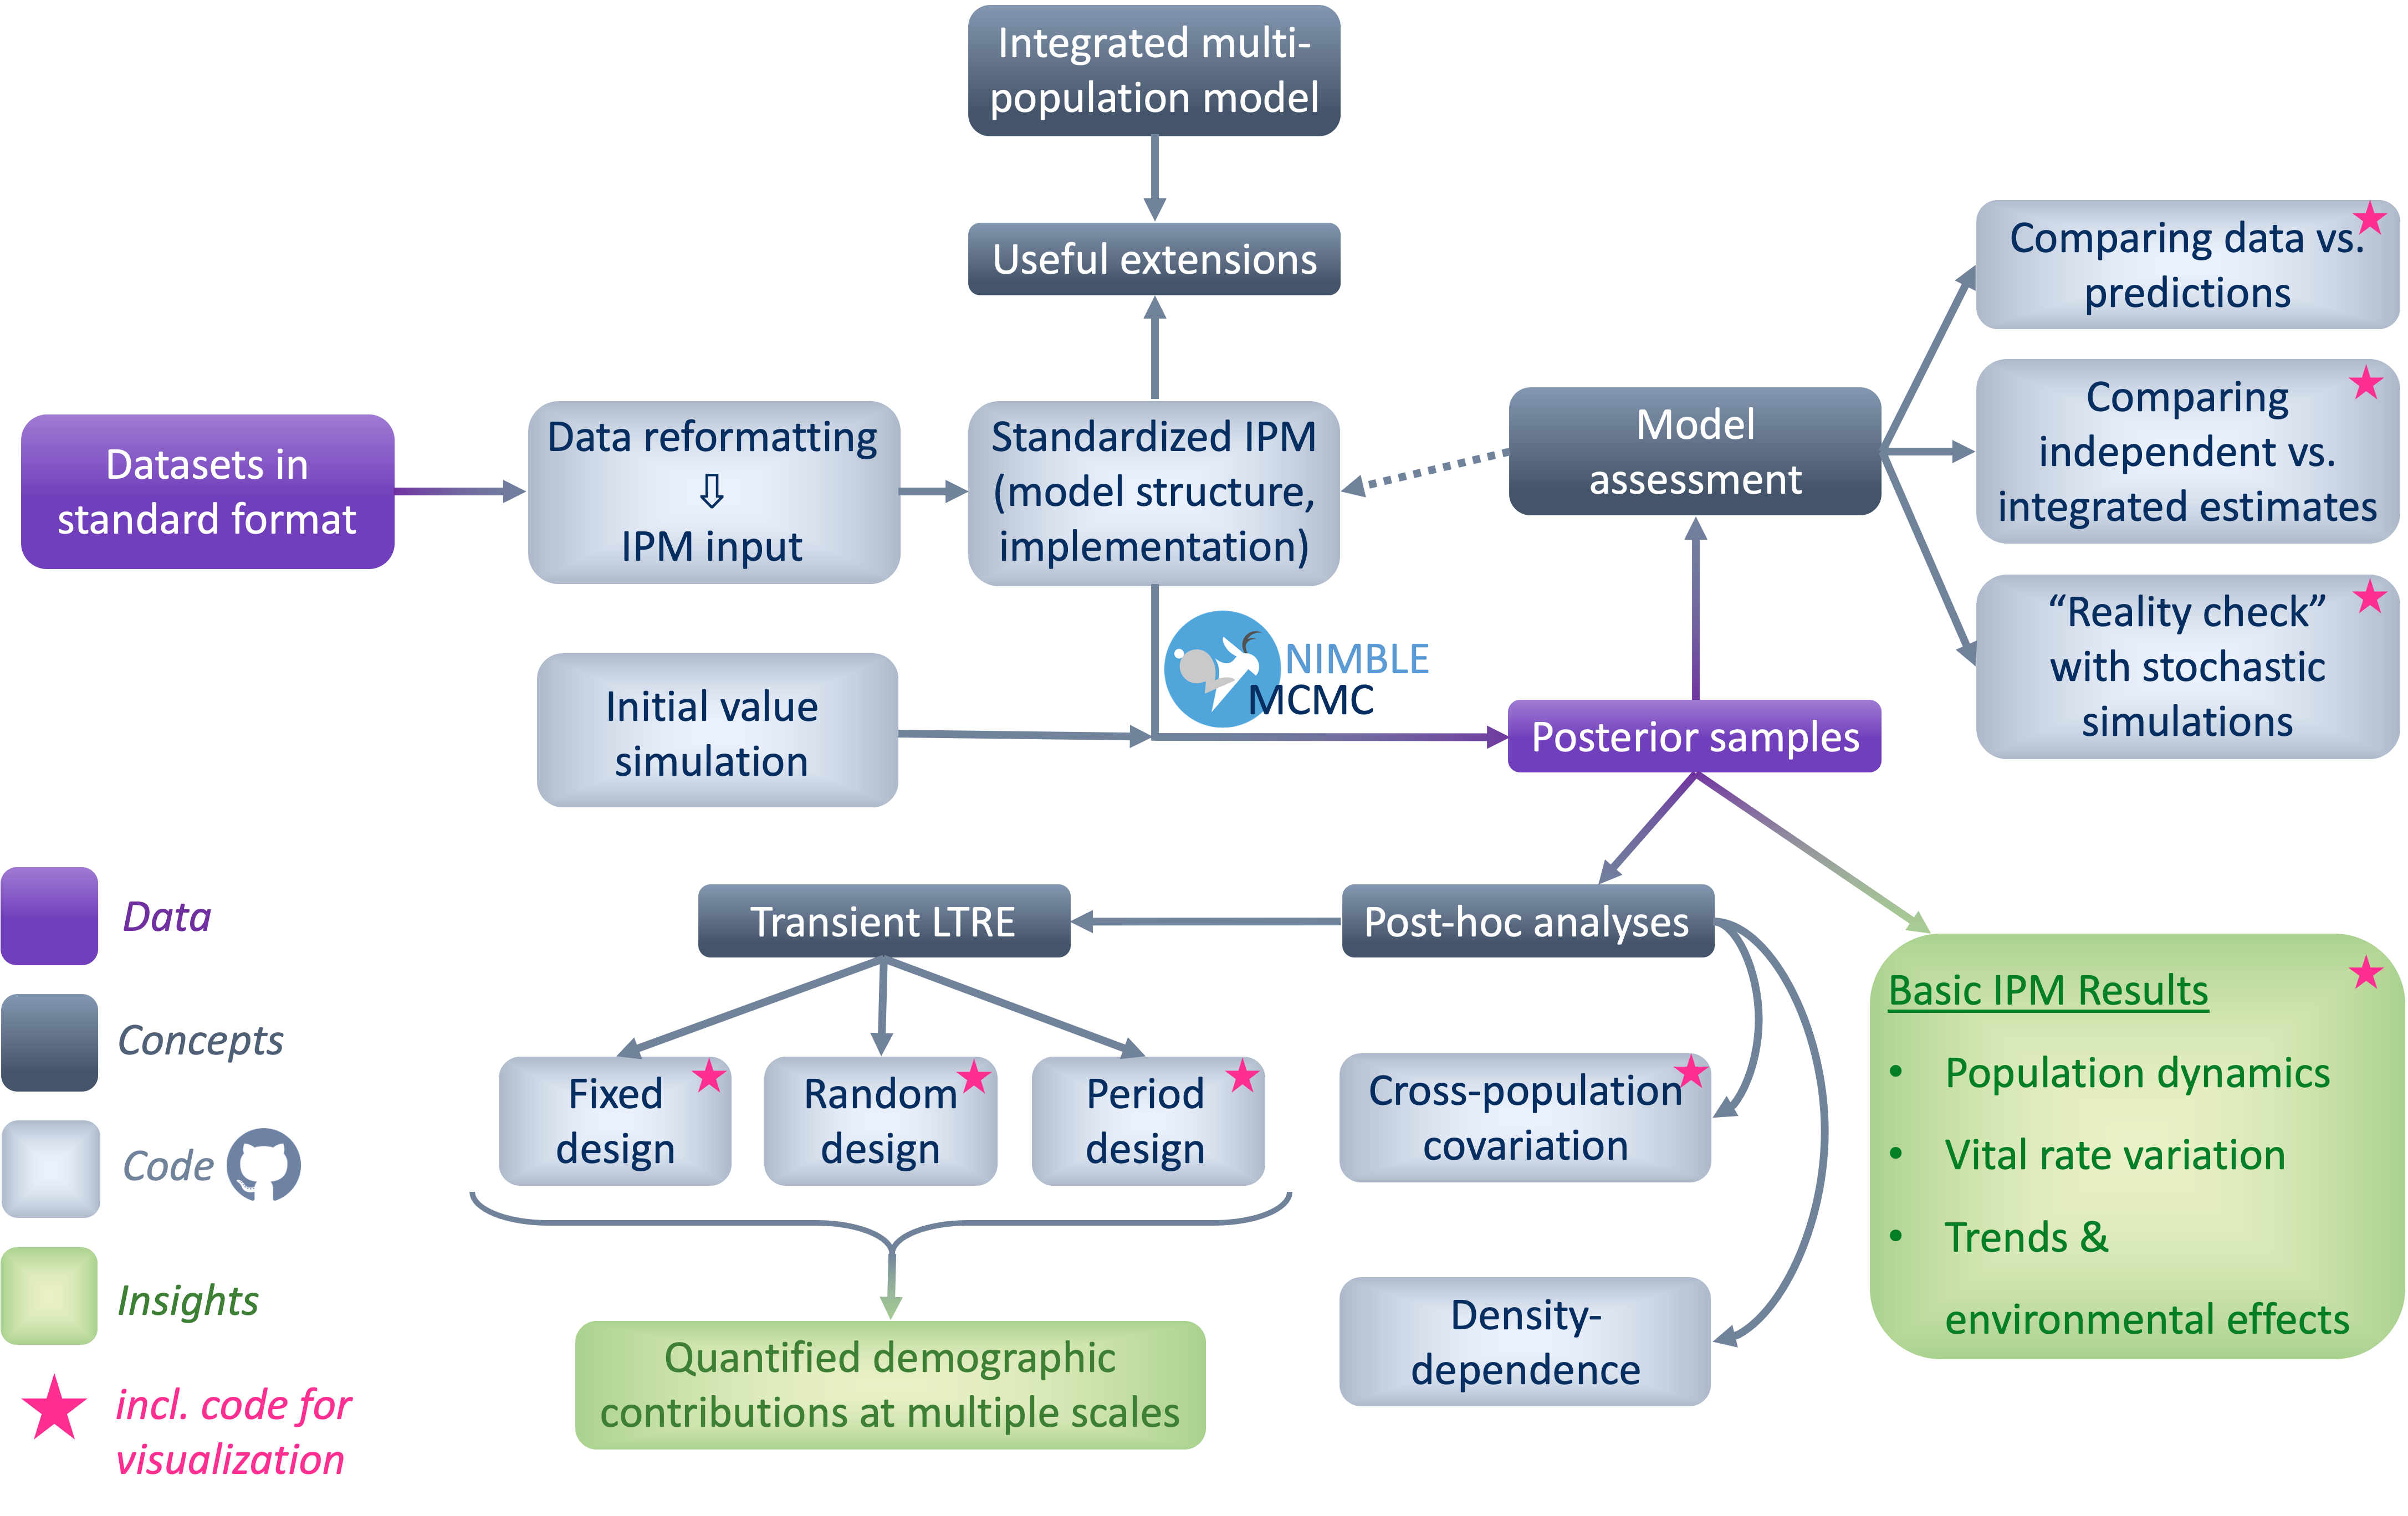
\includegraphics[width=1\linewidth]{Figures/SPI-IPM_Workflow} 

}

\caption{Schematic representation of the SPI-IPM workflow.}\label{fig:WorkflowDiag}
\end{figure}

In no way complete: great if user's analyses/adaptations become part.

How to cite.

\hypertarget{DataPrep}{%
\chapter{Preparing SPI-Birds data for Bayesian analysis}\label{DataPrep}}

Quick recap of SPI-Birds standard format and overview over data types used in IPM (+ how they relate, incl.~diagram).

\hypertarget{nest-count-data}{%
\section{Nest count data}\label{nest-count-data}}

\hypertarget{clutch-size-data}{%
\section{Clutch size data}\label{clutch-size-data}}

\hypertarget{nest-level}{%
\subsection{Nest level}\label{nest-level}}

\hypertarget{population-level}{%
\subsection{Population level}\label{population-level}}

\hypertarget{fledgling-count-data}{%
\section{Fledgling count data}\label{fledgling-count-data}}

\hypertarget{nest-level-1}{%
\subsection{Nest level}\label{nest-level-1}}

\hypertarget{population-level-1}{%
\subsection{Population level}\label{population-level-1}}

\hypertarget{mark-recapture-data}{%
\section{Mark-recapture data}\label{mark-recapture-data}}

\hypertarget{individual-capture-histories}{%
\subsection{Individual capture histories}\label{individual-capture-histories}}

\hypertarget{m-array}{%
\subsection{M-array}\label{m-array}}

\hypertarget{immigrant-count-data}{%
\section{Immigrant count data}\label{immigrant-count-data}}

\hypertarget{auxiliary-data-on-the-sampling-process}{%
\section{Auxiliary data on the sampling process}\label{auxiliary-data-on-the-sampling-process}}

\hypertarget{nest-survey-sampling-effort}{%
\subsection{Nest survey sampling effort}\label{nest-survey-sampling-effort}}

\hypertarget{capture-probability-proxies}{%
\subsection{Capture probability proxies}\label{capture-probability-proxies}}

\hypertarget{IPMCon}{%
\chapter{IPM Construction}\label{IPMCon}}

\hypertarget{open-population-model-with-2-age-classes}{%
\section{Open population model with 2 age classes}\label{open-population-model-with-2-age-classes}}

\hypertarget{model-description}{%
\subsection{Model description}\label{model-description}}

Population dynamics are represented using a female-based age-structured open
population model with a pre-breeding census in spring. At census, females are
divided into two age classes: ``yearlings'' (1-year old birds hatched during the
breeding season of the previous year) and ``adults'' (birds older than one year).
The motivation underlying this distinction is that reproductive output often
differs for these two age classes in passerine birds.
The dynamics of the female segment of the population over the time-interval from
census in year \(t\) to census in year \(t+1\) can be described with classic matrix
notation \citep{Caswell2001} as:

\[N_{tot,t+1} = \begin{bmatrix} N_{Y,t+1} \\ N_{A,t+1} \end{bmatrix} =
  \begin{bmatrix}
0.5F_{Y,t}sJ_t & 0.5F_{A,t}sJ_t \\
sA_t & sA_t
\end{bmatrix}\begin{bmatrix} N_{Y,t} \\ N_{A,t} \end{bmatrix} +
  \begin{bmatrix} Imm_{Y,t+1} \\ Imm_{A,t+1} \end{bmatrix}\]\\

\(N_{tot,t+1}\) represents the total number of yearling and adult females in the
population upon arrival in the breeding areas in year t. The total female
population size, \(N_{tot,t+1}\), is the sum of the numbers of yearling and adult
females in the population in year \(t+1\) (\(N_{Y,t+1}\) and \(N_{A,t+1}\),
respectively) and consists of local survivors and recruits from the previous
breeding season, as well as immigrant yearling (\(Imm_{Y,t+1}\)) and adult
(\(Imm_{A,t+1}\)) females.\\

\(F_{a,t}\) represents the expected number of fledglings produced by age class \(a\)
females during the breeding season in year \(t\) and is the product of several
vital rates. First, females in age class a may breed in a nestbox with
probability \(pB_{a,t}\) upon arrival to breeding areas in year \(t\). Each breeding
female may then lay a clutch containing a certain number of eggs (expected
number = \(CS_{a,t}\)), and each egg within the clutch may hatch and survive to
fledging. The probability of an egg hatching and surviving to fledging is
divided into an age-independent probability of nest success (\(pNS_t\),
probability of complete clutch failure = \(1-pNS_t\)) and a survival probability
of every egg/chick to fledging provided that the nest has not failed entirely
(\(sN_{a,t}\), with \(a\) = age of the mother). Consequently, the expected number of
fledglings produced by age class \(a\) females in year t is defined as:

\begin{equation}
F_{a,t}= pB_{a,t}\times CS_{a,t}\times pNS_{t}\times sN_{a,t}
\end{equation}

Fledglings that survive to the next breeding season and remain within the
population (probability = \(sJ_t\)) contribute to next year's yearling class
(\(N_{Y,t+1}\)). Yearlings and adults that survive to the next breeding season and
remain within the population (probability = \(sA_t\)) become part of next year's
adult age class (\(N_{A,t+1}\)).

\hypertarget{code-implementation-including-demographic-stochasticity}{%
\subsection{Code implementation including demographic stochasticity}\label{code-implementation-including-demographic-stochasticity}}

Population process models within IPMs are typically implemented as stochastic
models that account for randomness in the outcomes of demographic processes at
the individual level \citep[``demographic stochasticity'',][]{Caswell2001, kery2011}.
The model described here is no different, meaning that the numbers of breeders,
fledglings, and survivors are treated as binomial and Poisson random variables.

Reproduction is modelled via two sets of random variables: a binomial random
variable representing the number of breeders in age class \(a\) in year \(t\),
\(B_{a,t}\) and a Poisson random variable representing the
number of fledlings produced by breeders of age class \(a\) in year \(t\),
\(Juv_{a,t}\) . The implementation in the BUGS language used in the
SPI-IPM code (\href{https://github.com/SPI-Birds/SPI-IPM/blob/main/SPI-IPM_Code/02-04_IPM_Setup\&Run/IPMSetup.R}{\texttt{IPMSetup.R}}, lines 231-241) looks like:

\begin{Shaded}
\begin{Highlighting}[]
\ControlFlowTok{for}\NormalTok{ (t }\ControlFlowTok{in} \DecValTok{1}\OperatorTok{:}\NormalTok{Tmax)\{}
  \ControlFlowTok{for}\NormalTok{(a }\ControlFlowTok{in} \DecValTok{1}\OperatorTok{:}\NormalTok{A)\{}
    
    \CommentTok{## 1) Breeding decision}
\NormalTok{    B[a,t] }\OperatorTok{~}\StringTok{ }\KeywordTok{dbin}\NormalTok{(pB[a,t], N[a,t])}
    
    \CommentTok{## 2) Offspring production}
\NormalTok{    Juv[a,t] }\OperatorTok{~}\StringTok{ }\KeywordTok{dpois}\NormalTok{(B[a,t]}\OperatorTok{*}\NormalTok{CS[a,t]}\OperatorTok{*}\NormalTok{pNS[t]}\OperatorTok{*}\NormalTok{sN[a,t]}\OperatorTok{*}\FloatTok{0.5}\NormalTok{)}
\NormalTok{  \}}
\NormalTok{\}}
\end{Highlighting}
\end{Shaded}

In the code, the age indeces \(a=1\) and \(a=A=2\) correspond to yearlings and
adults, respectively.

Analogous to breeders, the numbers of local survivors -- both fledglings surviving their
first year and becoming yearlings, and yearlings and adults surviving to the
next year -- are implemented as binomial random variables (\href{https://github.com/SPI-Birds/SPI-IPM/blob/main/SPI-IPM_Code/02-04_IPM_Setup\&Run/IPMSetup.R}{\texttt{IPMSetup.R}}, lines 243-255):

\begin{Shaded}
\begin{Highlighting}[]
\ControlFlowTok{for}\NormalTok{ (t }\ControlFlowTok{in} \DecValTok{1}\OperatorTok{:}\NormalTok{(Tmax}\DecValTok{-1}\NormalTok{))\{}
  
  \CommentTok{## 3) Annual survival of local birds}
  \CommentTok{# Juveniles -> Yearlings}
\NormalTok{  localN[}\DecValTok{1}\NormalTok{,t}\OperatorTok{+}\DecValTok{1}\NormalTok{] }\OperatorTok{~}\StringTok{ }\KeywordTok{dbin}\NormalTok{(sJ[t], }\KeywordTok{sum}\NormalTok{(Juv[}\DecValTok{1}\OperatorTok{:}\NormalTok{A,t]))}
  \CommentTok{# Yearlings/Adults -> adults}
\NormalTok{  localN[}\DecValTok{2}\NormalTok{,t}\OperatorTok{+}\DecValTok{1}\NormalTok{] }\OperatorTok{~}\StringTok{ }\KeywordTok{dbin}\NormalTok{(sA[t], }\KeywordTok{sum}\NormalTok{(N[}\DecValTok{1}\OperatorTok{:}\NormalTok{A,t]))}
  
  \CommentTok{## 4) Immigration}
  \ControlFlowTok{for}\NormalTok{(a }\ControlFlowTok{in} \DecValTok{1}\OperatorTok{:}\NormalTok{A)\{}
\NormalTok{    N[a,t}\OperatorTok{+}\DecValTok{1}\NormalTok{] <-}\StringTok{ }\NormalTok{localN[a,t}\OperatorTok{+}\DecValTok{1}\NormalTok{] }\OperatorTok{+}\StringTok{ }\NormalTok{Imm[a,t}\OperatorTok{+}\DecValTok{1}\NormalTok{]}
\NormalTok{  \}}
\NormalTok{\}}
\end{Highlighting}
\end{Shaded}

Immigrant numbers are also treated as outcomes of stochastic processes, and
these are detailed in \protect\hyperlink{ux5cux23ux5cux23ux5cux2520Immigrantux5cux2520countux5cux2520dataux5cux2520likelihood}{2.2.5 Immigrant count data likelihood}.

\hypertarget{data-likelihoods}{%
\section{Data likelihoods}\label{data-likelihoods}}

IPMs obtain information on the population model's parameters (population sizes
and vital rates) from several different data sets. Information in each data set
is channeled into model parameters via one or multiple data likelihoods.\\
The SPI-IPM contains five data modules consisting of a total of eight data
likelihoods: nest count data (one likelihood), clutch size data (two likelihoods),
fledgling count data (three likelihoods), mark-recapture data (one likelihood),
and immigrant count data (one likelihood).
The likelihoods contained in each data module are described in detail in the
following sub-chapters. The underlying data sets are introduced in
\protect\hyperlink{DataPrep}{Chapter 1} of the manual.

\hypertarget{nest-count-data-likelihood}{%
\subsection{Nest count data likelihood}\label{nest-count-data-likelihood}}

The population model defines the true size of the female segment of the breeding
population in any year \(t\) via the year- and age-specific number of breeding
females:

\begin{equation}
B_{a,t}  \sim Binomial(N_{a,t}, pB_{a,t})
\end{equation}

The total size of the female breeding population (the sum of \(B_{a,t}\) over all
age classes) in year \(t\) is expected to correspond closely with the observed
number of first clutches laid in any year (\(NestCount_t\)).
The breeding population count thus contains information about both breeding
probability (\(pB_{a,t}\)) and population size (\(N_{a,t}\)) and its likelihood can
be defined as:

\begin{equation}
NestCount_t  \sim Poisson((B_{Y,t} + B_{A,t}) \times NS\_Data_t)
\end{equation}

Here, the year-specific variable \(NS\_Data_t\) is a correction factor introduced
for dealing with years in which no nest survey data was collected
(\(NestCount_t = 0\) due to lack of sampling). \(NS\_Data_t\) is set to 0 for years
without data collection, and to 1 in all other years.

The likelihood is written almost identically in the code, the only difference
being the use the \texttt{sum()} function over age classes \(1\) to \(A=2\) when
specifying the Poisson distribution (this provides more flexibility for
extending the model to more than two age classes):

\begin{Shaded}
\begin{Highlighting}[]
\ControlFlowTok{for}\NormalTok{(t }\ControlFlowTok{in} \DecValTok{1}\OperatorTok{:}\NormalTok{Tmax)\{}
\NormalTok{  NestCount[t] }\OperatorTok{~}\StringTok{ }\KeywordTok{dpois}\NormalTok{(}\KeywordTok{sum}\NormalTok{(B[}\DecValTok{1}\OperatorTok{:}\NormalTok{A,t])}\OperatorTok{*}\NormalTok{NS_Data[t])}
\NormalTok{\}}
\end{Highlighting}
\end{Shaded}

\hypertarget{clutch-size-data-likelihoods}{%
\subsection{Clutch size data likelihoods}\label{clutch-size-data-likelihoods}}

The counting of incubated eggs provides information about both individual-level
clutch size (\(CS_{a,t}\)) and reproductive output at the population level.
Consequently, two separate likelihoods can be specified for within the clutch
size data module.

Each individual clutch size observation can be treated as the outcome of a
Poisson process with an expected value of \(CS_{a,t}\) (where \(a\) is the age of
the female that laid the clutch, and \(t\) the year in which the clutch was laid).
In the code, the likelihood is formulated for each clutch size observation \(x\)
(out of a total of \texttt{CS\_X} observations) and includes nested indexing of the
expectation using data on female age (\texttt{CS\_FAge}) and year (\texttt{CS\_year}):

\begin{Shaded}
\begin{Highlighting}[]
\ControlFlowTok{for}\NormalTok{(x }\ControlFlowTok{in} \DecValTok{1}\OperatorTok{:}\NormalTok{CS_X)\{}
\NormalTok{    ClutchSize[x] }\OperatorTok{~}\StringTok{ }\KeywordTok{dpois}\NormalTok{(CS[CS_FAge[x], CS_year[x]])}
\NormalTok{\}}
\end{Highlighting}
\end{Shaded}

Since both year and female age need to be part of the provided data, the
individual-level clutch size likelihood can only be used with complete
observations, i.e.~clutches for which both number of eggs and age of the mother
are known (year should always be known).

For the population-level likelihood, on the other hand, data on clutch sizes can
be included irrespective of whether the age of the mother is known. The total
number of eggs counted in all nests laid in year \(t\) can be described as:

\begin{equation}
EggNoTot_t \sim Poisson(sum(B_{Y:A,t} \times CS_{Y:A,t}) \times p_t^{EggNo})
\end{equation}

Since the product \(B_{a,t} \times CS_{a,t}\) corresponds to all eggs laid in all nests/nestboxes within the study site, another correction factor (\(p_t^{EggNo}\)) is needed to account for the fact that eggs may not have been counted in all surveyed nests with breeding activity in each year. \(p_t^{EggNo}\) (\texttt{EggNoSP{[}t{]}} in code) thus contains information of the year-specific proportionof surveyed nests for which the numbers of eggs were counted.

In code, the likelihood for the number of eggs at the population is written as:

\begin{Shaded}
\begin{Highlighting}[]
\ControlFlowTok{for}\NormalTok{(t }\ControlFlowTok{in} \DecValTok{1}\OperatorTok{:}\NormalTok{Tmax)\{}

    \CommentTok{# Expected "true" egg number (by mother age class)}
\NormalTok{    EggNo.ex[}\DecValTok{1}\OperatorTok{:}\NormalTok{A,t] <-}\StringTok{ }\NormalTok{B[}\DecValTok{1}\OperatorTok{:}\NormalTok{A,t]}\OperatorTok{*}\NormalTok{CS[}\DecValTok{1}\OperatorTok{:}\NormalTok{A,t]}

    \CommentTok{# Observed egg number (corrected by data availaility)}
\NormalTok{    EggNoTot[t] }\OperatorTok{~}\StringTok{ }\KeywordTok{dpois}\NormalTok{(}\KeywordTok{sum}\NormalTok{(EggNo.ex[}\DecValTok{1}\OperatorTok{:}\NormalTok{A,t])}\OperatorTok{*}\NormalTok{EggNoSP[t])}

\NormalTok{\}}
\end{Highlighting}
\end{Shaded}

\hypertarget{fledgling-count-data-likelihoods}{%
\subsection{Fledgling count data likelihoods}\label{fledgling-count-data-likelihoods}}

Analogous to observations of clutch size, counts of fledglings contain
information on reproduction at both individual and population level.
Distributions of number of fledglings produced from a clutch are often 0-inflated
because incidents of harsh weather, predation, adandonment, etc. may result in
complete loss of entire clutches. To account for this, we split data on fledgling
numbers and formulated separate likelihoods for the survival of the clutch as
a whole (probability of a nest not failing completely, \(pNS_t\)) and for each
chick subsequently surviving to fledgling (probability \(sN_{a,t}\)).\\
Whether or not a clutch succeeded (i.e.~at least one chick survived to fledging,
\texttt{anyFledged}) was coded using 1 (success) and 0 (failure) and modelled as the
outcome of a Bernoulli process with a year-dependent success probability \(pNS_t\):

\begin{Shaded}
\begin{Highlighting}[]
\ControlFlowTok{for}\NormalTok{(x }\ControlFlowTok{in} \DecValTok{1}\OperatorTok{:}\NormalTok{F_X)\{}
\NormalTok{  anyFledged[x] }\OperatorTok{~}\StringTok{ }\KeywordTok{dbern}\NormalTok{(pNS[F_year[x]])}
\NormalTok{\}}
\end{Highlighting}
\end{Shaded}

For the subset of successful clutches, the number of fledglings produced
(\texttt{NoFledged}) was modelled as a binomial random variable with each egg laid in
the clutch (\texttt{NoLaid}) having a probability of \(sN_{a,t}\) (where \(a\) = age of the
mother) to survive and fledge:

\begin{Shaded}
\begin{Highlighting}[]
\ControlFlowTok{for}\NormalTok{(x }\ControlFlowTok{in} \DecValTok{1}\OperatorTok{:}\NormalTok{NoF_X)\{}
\NormalTok{    NoFledged[x] }\OperatorTok{~}\StringTok{ }\KeywordTok{dbin}\NormalTok{(sN[NoF_FAge[x], NoF_year[x]], NoLaid[x])}
\NormalTok{\}}
\end{Highlighting}
\end{Shaded}

At the population level, both processes (nest success and survival to fledging
conditional on nest success) were combined into a single Poisson
likelihood describing the total number of fledglings counted in the population
in a given year \(t\) as the product of the number of breeding females, clutch
size, nest success, and survival to fledging:

\begin{equation}
FledgedTot_t  \sim Poisson(sum(B_{Y:A,t}\times CS_{Y:A,t}\times pNS_t\times sN_{Y:A,t}) \times p_t^{Fledged})
\end{equation}

As in the clutch size data module (\protect\hyperlink{ux5cux23ux5cux23ux5cux2520Clutchux5cux2520sizeux5cux2520dataux5cux2520likelihoods}{Chapter 2.2.2}),
a correction factor quantifying the proportion of nests for which data is
availeble (\(p_t^{Fledged}\), \texttt{FledgedSP{[}t{]}} in code) is used to account for
missing records of fledgling numbers.

In the code, calculation of the expected number of fledglings is based on the expected number of eggs as calculated in the clutch size data module
(\protect\hyperlink{ux5cux23ux5cux23ux5cux2520Clutchux5cux2520sizeux5cux2520dataux5cux2520likelihoods}{Chapter 2.2.2}):

\begin{Shaded}
\begin{Highlighting}[]
\ControlFlowTok{for}\NormalTok{(t }\ControlFlowTok{in} \DecValTok{1}\OperatorTok{:}\NormalTok{Tmax)\{}

    \CommentTok{# Expected "true" fledgling number (by mother age class)}
\NormalTok{    Fledged.ex[}\DecValTok{1}\OperatorTok{:}\NormalTok{A,t] <-}\StringTok{ }\NormalTok{EggNo.ex[}\DecValTok{1}\OperatorTok{:}\NormalTok{A,t]}\OperatorTok{*}\NormalTok{pNS[t]}\OperatorTok{*}\NormalTok{sN[}\DecValTok{1}\OperatorTok{:}\NormalTok{A,t]}

    \CommentTok{# Observed egg number (corrected by data availaility)}
\NormalTok{    FledgedTot[t] }\OperatorTok{~}\StringTok{ }\KeywordTok{dpois}\NormalTok{(}\KeywordTok{sum}\NormalTok{(Fledged.ex[}\DecValTok{1}\OperatorTok{:}\NormalTok{A,t])}\OperatorTok{*}\NormalTok{FledgedSP[t])}
\NormalTok{\}}
\end{Highlighting}
\end{Shaded}

\hypertarget{mark-recapture-data-likelihood}{%
\subsection{Mark-recapture data likelihood}\label{mark-recapture-data-likelihood}}

In the SPI-IPM, capture histories of marked birds are analysed using an age-specific Cormack-Jolly-Seber (CJS) model \citep{cormack1964, jolly1965, seber1965}, which allows estimation of parameters associated with both annual survival and the (re-)capturing process.\\
The survival parameters \(sJ_t\) and \(sA_t\) describe the probability of surviving from one breeding season to the next for fledglings/juveniles and adult females, respectively. Since field-based sexing fledglings is not possible in the hatch year, first-year survival in the CJS likelihood was set to \(0.5sJ_t\), representing the probability that a fledgling is female and survives (recaptures of adult males were removed from the capture histories).\\
The time- and age-dependent recapture parameters \(p_{Age,t}^{Recap}\) describe the probability that an age class \(a\) individual is recaptured and identified during the breeding season of year \(t\) given that it survived the time interval \(t-1\) to \(t\). For many of the bird populations included in SPI-Birds, (re-)captures of birds are carried out at the nestboxes during the breeding season only. Consequently, two conditions need to be met for a (re-)capture besides the individual being alive: 1) the individual breeds in a nestbox (as non-breeders and birds breeding in natural cavities are not captured) and 2) the individual is actually captured and marked/identified while breeding in a nestbox. The recapture probability is therefore the product of the probability of breeding in a nestbox (\(pB_{Age,t}\)) and the probability of capture and identification given breeding in a nestbox (\(p_t^{CapB}\)):
\begin{equation}
  p_{Age,t}^{Recap}=pB_{Age,t}\times p_t^{CapB}
\end{equation}
The parameters \(pB_{Age,t}\) and \(p_t^{CapB}\) are confounded, and auxiliary data on one of them is required to separately estimate them. Here, raw data on the annual proportions of surveyed nests for which the identity of the breeding female was recorded (as a result of ringing or recapture) is used to approximated \(p_t^{CapB}\), allowing the CJS model to estimate age- and time-specific breeding probabilities (\(pB_{Age,t}\)).\\
CJS models in Bayesian frameworks have traditionally been implemented either as latent states models with Bernouilli likelihoods or as multinomial likelihoods for data re-formatted as ``m-arrays'' \citep{gimenez2007, kery2011}. The former typically results in long runtimes and high computational costs, while the improved efficiency of the latter is tied to an implementation that suffers from being neither particularly intuitive nor user-friendly. To avoid these pitfalls, the CJS model in the SPI-IPM is implemented using a much more efficient marginalized likelihood (that integrates over all latent states) that can be applied to unique (not individual) capture histories only \citep[following][]{turek2016}:

\begin{Shaded}
\begin{Highlighting}[]
\CommentTok{## Likelihood with custom distribution}
\ControlFlowTok{for}\NormalTok{ (i }\ControlFlowTok{in} \DecValTok{1}\OperatorTok{:}\NormalTok{n.CH)\{}

\NormalTok{  y.sum[i, first.sum[i]}\OperatorTok{:}\NormalTok{last.sum[i]] }\OperatorTok{~}\StringTok{ }\KeywordTok{dCJS_vv_sum}\NormalTok{(}
      \DataTypeTok{probSurvive =}\NormalTok{ phi.CH[i, first.sum[i]}\OperatorTok{:}\NormalTok{last.sum[i]],}
      \DataTypeTok{probCapture =}\NormalTok{ p.CH[i, first.sum[i]}\OperatorTok{:}\NormalTok{last.sum[i]],}
      \DataTypeTok{len =}\NormalTok{ last.sum[i]}\OperatorTok{-}\NormalTok{first.sum[i]}\OperatorTok{+}\DecValTok{1}\NormalTok{,}
      \DataTypeTok{mult =}\NormalTok{ CHs.count[i])}
\NormalTok{    \}}
\end{Highlighting}
\end{Shaded}

In practice, this involves the use of a custom distribution \texttt{dCJS\_vv\_sum}, and more information on the likelihood and its implementation using NIMBLE is provided in \protect\hyperlink{ux5cux23ux5cux2520Efficientux5cux2520implementationux5cux2520usingux5cux2520NIMBLE}{Chapter 4.1 (Efficient implementation using NIMBLE)}.

\hypertarget{immigrant-count-data-likelihood}{%
\subsection{Immigrant count data likelihood}\label{immigrant-count-data-likelihood}}

In many nestbox studies, chick ringing is an exhaustive effort and it is not unreasonable to assume that all chicks hatched in nestboxes within a study population are ringed before fledging. Similarly, assuming that females captured in nestboxes are breeding (or attempting to breed) is often not far from the truth. If those two assumptions are largely met, then the annual numbers of newly ringed adult females (\(ImmNoObs_t\)) can provide information about immigration or -- more specifically -- about the latent number of newly immigrated females breeding in nestboxes each year (\(ImmNoTot_t\)). Typically, age will be unknown for immigrant females (unless they were marked as chicks elsewhere) and hence there is no age index on \(ImmNoObs_t\) and \(ImmNoTot_t\). In \texttt{SPI-IPM}, we use a Poisson observation model to describe the relationship between observed and true numbers of breeding immigrant females:
\begin{equation}
  ImmNoObs_t \sim Poisson(ImmNoTot_t \times p_t^{ImmDetect})
\end{equation}
The expected value represents the true number of female breeding immigrants in year \(t\) (\(ImmNoTot_t\)) corrected by an annual probability of detecting (= ringing) such individuals (\(p_t^{ImmDetect}\)). In most nestbox studies, ringing and recapturing of breeding birds are conducted in tandem as part of the same protocol, and we can consequently approximate adult ringing probability using recapture probability (as used in the likelihood for capture histories): \(p_t^{ImmDetect} = p_t^{CapB}\)). In a few exceptional years in some datasets, however, adult birds may have been ringed, but no recaptures recorded (i.e.~\(p_t^{CapB}=0\) but \(p_t^{ImmDetect}>0\)). These cases call for estimation of (or, in other words, accounting for the uncertainty in) the corresponding \(p_t^{ImmDetect}>0\). As long as such cases are relatively few, this can be accommodated by specifying a non-informative prior for the unknown value\footnote{For estimating only a subset of values within a vector/array (= partially observed variables), data (here \texttt{PropImmDetect{[}t{]}}) is provided including \texttt{NA} for unknown values and initial values are provided for the corresponding indeces (with initial values matching indeces of known data points being set to \texttt{NA}). Handling partially observed variables is discussed some more under \protect\hyperlink{ux5cux23ux5cux23ux5cux2520Imputationux5cux2520ofux5cux2520missingux5cux2520covariateux5cux2520values}{3.2.3 Imputation of missing covariate values}}:

\begin{Shaded}
\begin{Highlighting}[]
\CommentTok{## Immigrant detection (= marking) probability}
  \ControlFlowTok{for}\NormalTok{(t }\ControlFlowTok{in} \DecValTok{1}\OperatorTok{:}\NormalTok{Tmax)\{}
\NormalTok{    PropImmDetect[t] }\OperatorTok{~}\StringTok{ }\KeywordTok{dunif}\NormalTok{(}\DecValTok{0}\NormalTok{, }\DecValTok{1}\NormalTok{)}
\NormalTok{  \}}
\end{Highlighting}
\end{Shaded}

The latent number of breeding immigrants, informed by data as outlined above, is estimated as pooled across age classes (\(ImmNoTot_t\)), but the since the population model in \texttt{SPI-IPM} is age structured \(ImmNoTot_t = ImmB_{Y,t} +ImmB_{A,t}\), where \(ImmB_{Y,t}\) and \(ImmB_{A,t}\) the numbers of breeding yearling and adult immigrants, respectively. These quantities are linked to the total numbers of immigrants in each age class (breeding and non-breeding), \(Imm_{a,t}\), that appear in the age-structured population model (\protect\hyperlink{ux5cux23ux5cux2520Openux5cux2520populationux5cux2520modelux5cux2520withux5cux25202ux5cux2520ageux5cux2520classes}{Chapter 2.1} through age-specific breeding probabilities.
By assuming equal breeding probabilities for locally recruited and newly immigrated females, we can use the breeding probabilities estimated via the mark-recapture likelihood (\(pB_{a,t}\)) to make the connection:
\begin{equation}
  ImmB_{a,t} \sim Binomial(Imm_{a,t}, pB_{a,t})
\end{equation}

In the code, the sub-model for immigration contains both the likelihood for the immigrant count data pooled across ages and the relationship between breeding immigrant females and all immigrant females in both age classes:

\begin{Shaded}
\begin{Highlighting}[]
\CommentTok{## Likelihood for the number/age distribution of immigrant females}
\ControlFlowTok{for}\NormalTok{ (t }\ControlFlowTok{in} \DecValTok{2}\OperatorTok{:}\NormalTok{Tmax)\{}

  \CommentTok{# Latent true number of breeding immigrants (count observation model)}
\NormalTok{  ImmNoObs[t] }\OperatorTok{~}\StringTok{ }\KeywordTok{dpois}\NormalTok{(}\KeywordTok{sum}\NormalTok{(ImmB[}\DecValTok{1}\OperatorTok{:}\NormalTok{A,t])}\OperatorTok{*}\NormalTok{PropImmDetect[t])}

  \CommentTok{# Number of breeding immigrants per age class}
  \ControlFlowTok{for}\NormalTok{(a }\ControlFlowTok{in} \DecValTok{1}\OperatorTok{:}\NormalTok{A)\{}
\NormalTok{    ImmB[a,t] }\OperatorTok{~}\StringTok{ }\KeywordTok{dbin}\NormalTok{(pB[a,t], Imm[a,t])}
\NormalTok{  \}}
\NormalTok{\}}

\NormalTok{ImmNoObs[}\DecValTok{1}\NormalTok{] <-}\StringTok{ }\DecValTok{0}
\NormalTok{ImmB[}\DecValTok{1}\OperatorTok{:}\NormalTok{A,}\DecValTok{1}\NormalTok{] <-}\StringTok{ }\DecValTok{0}
\end{Highlighting}
\end{Shaded}

Note that various immigrant numbers are set to 0 at \(t=1\) since there is no way of distinguishing between locally-born and newly immigrated birds in the first year of study.

\hypertarget{priors-and-constraints}{%
\section{Priors and constraints}\label{priors-and-constraints}}

In the model description above, all vital rate parameters, as well as initial
population size and immigrant numbers, appear as fully time- and age-dependent
parameters (i.e.~indexed by \(t\) = year and \(a\) = age class). \texttt{SPI-IPM} is a
hierarchical model, meaning it also describes how demographic quantities vary
across time and age classes and requires priors for the parameters defining
these underlying processes. The priors in the model's standard implementation
are all non- or only weakly informative, but they can easily be replaced with
more informative priors if required (see e.g.~Chapter \protect\hyperlink{ux5cux23ux5cux2520Includingux5cux2520additionalux5cux2520dataux5cux2520andux5cux2520informativeux5cux2520priors}{8.2}).

Time- and age-dependence in all vital rates is expressed using generalized
mixed-effect models. The exact model structure for each vital rate,
including link function, is described in detail in Chapter \protect\hyperlink{ux5cux2520Modellingux5cux2520temporalux5cux2520variation}{3}. Irrespective of the vital rate, the basic model parameters fall into
three categories: (age-specific) intercepts representing time-average vital
rates (\(\mu\)), slope parameters for the effects of temporal covariates (\(\beta\)),
and standard deviations describing the distribution of random year effects
(\(\sigma\)).
The intercept parameters \(\mu\) are defined on the natural scale to allow for
more intuitive setting of priors. As such, non-informative Uniform(0,1) priors
can be used for the \(\mu\) of all vital rates representing probabilities
(\(\mu_a^{pB}\), \(\mu^{pNS}\), \(\mu_a^{sN}\), \(\mu^{sJ}\), and \(\mu^{sA}\)). For the
age-specific average clutch size (\(\mu_a^{CS}\)), we use a Uniform(0,10) prior.
This latter prior is not completely uninformative, as it sets an upper limit of
10 eggs for the average clutch size (this is reasonable for pied flycatchers
\textit{Ficedula hypoleuca} for which \texttt{SPI-IPM} was initially developed, but
may have to be adjusted for species that lay larger clutches).
All slope parameters \(\beta\) are given Uniform(-5,5) priors, and all \(\sigma\)
parameters (except for the one linked to immigration, \(\sigma_a^{Imm}\)) are
given Uniform(0,10) priors.

Priors and constraints are also required for the initial population size, i.e.
\(N_{Y,1}\) and \(N_{A,1}\) since the population process model only begins
predicting \(N\) from the second year (\(t=2\)) onward. Immigrant numbers have their
own set of priors (see below), and since \(N_{a,t} = localN_{a,t} + Imm_{a,t}\),
priors have to be set for \(localN_{a,1}\) specifically. \texttt{SPI-IPM} uses what is
essentially a discrete uniform prior for initial local population size:

\begin{Shaded}
\begin{Highlighting}[]
     \CommentTok{## Initial population sizes}

     \ControlFlowTok{for}\NormalTok{(a }\ControlFlowTok{in} \DecValTok{1}\OperatorTok{:}\NormalTok{A)\{}
\NormalTok{        localN[a,}\DecValTok{1}\NormalTok{] }\OperatorTok{~}\StringTok{ }\KeywordTok{dcat}\NormalTok{(DU.prior[}\DecValTok{1}\OperatorTok{:}\NormalTok{N1.limit])}
\NormalTok{      N[a,}\DecValTok{1}\NormalTok{] <-}\StringTok{ }\NormalTok{localN[a,}\DecValTok{1}\NormalTok{] }\OperatorTok{+}\StringTok{ }\NormalTok{Imm[a,}\DecValTok{1}\NormalTok{]}
\NormalTok{     \}}

\NormalTok{     DU.prior[}\DecValTok{1}\OperatorTok{:}\NormalTok{N1.limit] <-}\StringTok{ }\DecValTok{1}\OperatorTok{/}\NormalTok{N1.limit}
\end{Highlighting}
\end{Shaded}

Here, \texttt{N1.limit} is a user-specified maximum possible number of local females in
any age class at the first time-step. The discrete uniform distribution is
approximated using a categorical distribution in which each integer number between
1 and \texttt{N1.limit} has the same probability (\texttt{1/N1.limit}) of occurring.
This approach is equivalent to using a regular Uniform(0,\texttt{N1.limit}) distribution
and subsequently rounding it.

The final set of priors and constraints in the model are for immigrant numbers
\(Imm_{Y,t}\) and \(Imm_{A,t}\). At the first time-step (\(t=1\)), immigrant numbers
are set to 0 (since there is no way of distinguishing previously local and
newly immigrated individuals in the first year of a study). Numbers at any
subsequent time-step are assumed to follow a 0-truncated normal distribution
with age-specific mean \(AvgImm_a\) (\texttt{AvgImm{[}a{]}}) and standard deviation
\(\sigma_a^{Imm}\) (\texttt{sigma.Imm{[}a{]})}):

\begin{Shaded}
\begin{Highlighting}[]
     \CommentTok{## Latent number of all immigrants (breeding & non-breeding) per age class}
\NormalTok{     Imm[}\DecValTok{1}\OperatorTok{:}\NormalTok{A,}\DecValTok{1}\NormalTok{] <-}\StringTok{ }\DecValTok{0}

     \ControlFlowTok{for}\NormalTok{(t }\ControlFlowTok{in} \DecValTok{2}\OperatorTok{:}\NormalTok{Tmax)\{}
       \ControlFlowTok{for}\NormalTok{(a }\ControlFlowTok{in} \DecValTok{1}\OperatorTok{:}\NormalTok{A)\{}

\NormalTok{         ImmCont[a,t] }\OperatorTok{~}\StringTok{ }\KeywordTok{T}\NormalTok{(}\KeywordTok{dnorm}\NormalTok{(AvgImm[a], }\DataTypeTok{sd =}\NormalTok{ sigma.Imm[a]), }\DecValTok{0}\NormalTok{, }\OtherTok{Inf}\NormalTok{)}
\NormalTok{         Imm[a,t] <-}\StringTok{ }\KeywordTok{round}\NormalTok{(ImmCont[a,t])}
\NormalTok{       \}}
\NormalTok{     \}}
\end{Highlighting}
\end{Shaded}

The rounding function ensures that immigrant numbers are integers.
Priors are then required for \(AvgImm_a\) and \(\sigma_a^{Imm}\), and these are
given as uniform distributions with values ranging from 0 to (a multiple of) a
user-specified maximum possible number of immigrant females in any age class:

\begin{Shaded}
\begin{Highlighting}[]
\ControlFlowTok{for}\NormalTok{(a }\ControlFlowTok{in} \DecValTok{1}\OperatorTok{:}\NormalTok{A)\{}
\NormalTok{  AvgImm[a] }\OperatorTok{~}\StringTok{ }\KeywordTok{dunif}\NormalTok{(}\DecValTok{0}\NormalTok{, AvgImm.limit)}
\NormalTok{  sigma.Imm[a] }\OperatorTok{~}\StringTok{ }\KeywordTok{dunif}\NormalTok{(}\DecValTok{0}\NormalTok{, AvgImm.limit}\OperatorTok{*}\DecValTok{10}\NormalTok{)}
\NormalTok{\}}
\end{Highlighting}
\end{Shaded}

\hypertarget{TempVar}{%
\chapter{Modelling temporal variation}\label{TempVar}}

Vital rates are expected to vary among years due to changes in environmental
conditions. \texttt{SPI-IPM} is set up to account for among-year variation in
different (age-specific) vital rates \(X_{a,t}\) using fixed effects of
supplied environmental covariates (\(cov1_t\), \(cov2_t\),\ldots) and year random effects (\(\epsilon_t^X\)). The resulting generalized linear
mixed-models for time- and age-specific vital rates therefore take the following
form:
\begin{equation}
  link(X_{a,t}) = link(\mu_a^X) + \beta_{cov1}^X\times cov1_t + \beta_{cov2}^X\times cov2_t + ... + \epsilon_t^X
\end{equation}
Here, \(\mu_a^X\) is the age-specific average vital rate (intercept) and \(\beta_{cov1}\)
and \(\beta_{cov2}\) are the slopes for the effects of covariates \(cov1\) and \(cov2\)
on the link scale, respectively.
The link function depends on the vital rate, and is set to logit for breeding
probabilities (\(pB_{a,t}\)), nest success probabilities (\(pNS_t\)), and survival
probabilities (\(sN_{a,t}\), \(sJ_t\), \(sA_t\)) and log for clutch size (\(CS_{a,t}\)).

\hypertarget{random-year-variation}{%
\section{Random year variation}\label{random-year-variation}}

The random year effects included in the basic implementation of \texttt{SPI-IPM} are
assumed to be normally distributed such that
\begin{equation}
  \epsilon_{t}^X \sim Normal(0, \sigma^X)
\end{equation}
where \(\sigma^X\) is the standard deviation of random year effects on vital rate
\(X_{a,t}\).
The random effects in the basic implementation are also age-independent, meaning
that \(\epsilon_t^X\) is included in the equations for both the yearling vital
rate \(X_{Y,t}\) and the adults vital rate \(X_{A,t}\). The exception are the annual
survival rates for juveniles (\(sJ_t\)) and (\(sA_t\)), which both have separate
random effects because the drivers of survival variation are expected to vary
between those two age classes, and the basic implementation includes an
additional covariate effect \(sJ_t\) only:

\begin{Shaded}
\begin{Highlighting}[]
\CommentTok{## Age- and time-dependent survival probabilities}
\KeywordTok{logit}\NormalTok{(sJ[}\DecValTok{1}\OperatorTok{:}\NormalTok{Tmax]) <-}\StringTok{ }\KeywordTok{logit}\NormalTok{(Mu.sJ) }\OperatorTok{+}\StringTok{ }\NormalTok{beta3.sJ}\OperatorTok{*}\NormalTok{cov3[}\DecValTok{1}\OperatorTok{:}\NormalTok{Tmax] }\OperatorTok{+}\StringTok{ }\NormalTok{epsilon.sJ[}\DecValTok{1}\OperatorTok{:}\NormalTok{Tmax]}
\KeywordTok{logit}\NormalTok{(sA[}\DecValTok{1}\OperatorTok{:}\NormalTok{Tmax]) <-}\StringTok{ }\KeywordTok{logit}\NormalTok{(Mu.sA) }\OperatorTok{+}\StringTok{ }\NormalTok{epsilon.sA[}\DecValTok{1}\OperatorTok{:}\NormalTok{Tmax]}

\CommentTok{## Temporal random effects}
\ControlFlowTok{for}\NormalTok{(t }\ControlFlowTok{in} \DecValTok{1}\OperatorTok{:}\NormalTok{Tmax)\{}
\NormalTok{     epsilon.sJ[t] }\OperatorTok{~}\StringTok{ }\KeywordTok{dnorm}\NormalTok{(}\DecValTok{0}\NormalTok{, }\DataTypeTok{sd =}\NormalTok{ sigma.sJ)}
\NormalTok{     epsilon.sA[t] }\OperatorTok{~}\StringTok{ }\KeywordTok{dnorm}\NormalTok{(}\DecValTok{0}\NormalTok{, }\DataTypeTok{sd =}\NormalTok{ sigma.sA)}
\NormalTok{\}}
\end{Highlighting}
\end{Shaded}

All random effects are treated as independent (= not correlated) in the basic
implementation of the model, but the inclusion of correlation of random effects
across age-classes and/or vital rates is straightforward to implement\footnote{Wheter or
  not formally including random effects correlations is useful or not depends on
  the biological questions of interest and the amoung of data available. When
  testing a model with correlated random effects for juvenile and adult survival
  on seven datasets from breeding populations of pied flycatchers in the UK, I
  found that estimates did not differ from those obtained from a model with
  independent random effects, and the posterior distribution for the correlation
  coefficient was so wide that no inference on strength or direction of the
  correlation was possible.} using e.g.
multivariate normal distributions or approaches similar to the one used in
\citet{nater2020}.

\hypertarget{temporal-covariates}{%
\section{Temporal covariates}\label{temporal-covariates}}

\hypertarget{continuous-variables}{%
\subsection{Continuous variables}\label{continuous-variables}}

\hypertarget{categorical-variables}{%
\subsection{Categorical variables}\label{categorical-variables}}

\hypertarget{imputation-of-missing-covariate-values}{%
\subsection{Imputation of missing covariate values}\label{imputation-of-missing-covariate-values}}

\hypertarget{notes-on-covariate-selection}{%
\chapter{\#\# Notes on covariate selection}\label{notes-on-covariate-selection}}

\hypertarget{tba-later}{%
\chapter{{[}TBA later{]}}\label{tba-later}}

\hypertarget{IPMImp}{%
\chapter{IPM Implementation}\label{IPMImp}}

\hypertarget{efficient-implementation-using-nimble}{%
\section{Efficient implementation using NIMBLE}\label{efficient-implementation-using-nimble}}

We use the fantastic \textbf{nimble} package \citep{devalpine2017}!

\hypertarget{simulation-of-initial-values}{%
\section{Simulation of initial values}\label{simulation-of-initial-values}}

\hypertarget{test-runs-and-full-runs-chains-iterations-burn-in-and-thinning}{%
\section{Test runs and full runs: chains, iterations, burn-in, and thinning}\label{test-runs-and-full-runs-chains-iterations-burn-in-and-thinning}}

\hypertarget{trouble-shooting-implementation-issues}{%
\section{Trouble-shooting implementation issues}\label{trouble-shooting-implementation-issues}}

\hypertarget{ModelAssm}{%
\chapter{Model Assessment}\label{ModelAssm}}

\hypertarget{assessing-chain-convergence}{%
\section{Assessing chain convergence}\label{assessing-chain-convergence}}

\hypertarget{plotting-data-vs.-predictions}{%
\section{Plotting data vs.~predictions}\label{plotting-data-vs.-predictions}}

\hypertarget{comparing-estimates-from-integrated-vs.-independent-analyses}{%
\section{Comparing estimates from integrated vs.~independent analyses}\label{comparing-estimates-from-integrated-vs.-independent-analyses}}

\hypertarget{reality-check-using-stochastic-simulations}{%
\section{``Reality check'' using stochastic simulations}\label{reality-check-using-stochastic-simulations}}

\hypertarget{other-approaches}{%
\section{Other approaches}\label{other-approaches}}

Running for additional years and comparing to non-included data, PPCs, etc.

\hypertarget{ResultsViz}{%
\chapter{Visualizing and interpreting direct IPM outputs}\label{ResultsViz}}

\hypertarget{population-trajectories}{%
\section{Population trajectories}\label{population-trajectories}}

\hypertarget{within-population-variation-in-vital-rates}{%
\section{Within-population variation in vital rates}\label{within-population-variation-in-vital-rates}}

\hypertarget{age-class-specific-averages}{%
\subsection{Age-class-specific averages}\label{age-class-specific-averages}}

\hypertarget{year-by-year-variation}{%
\subsection{Year-by-year variation}\label{year-by-year-variation}}

\hypertarget{between-population-variation-in-vital-rates}{%
\section{Between-population variation in vital rates}\label{between-population-variation-in-vital-rates}}

\hypertarget{population-specific-averages}{%
\subsection{Population-specific averages}\label{population-specific-averages}}

\hypertarget{year-by-year-variation-1}{%
\subsection{Year-by-year variation}\label{year-by-year-variation-1}}

\hypertarget{covariate-effects}{%
\section{Covariate effects}\label{covariate-effects}}

\hypertarget{AddAnalyses}{%
\chapter{Follow-up Analyses}\label{AddAnalyses}}

\hypertarget{testing-for-time-trends}{%
\section{Testing for time-trends}\label{testing-for-time-trends}}

\hypertarget{testing-for-density-dependence}{%
\section{Testing for density-dependence}\label{testing-for-density-dependence}}

\hypertarget{investigating-cross-population-covariation}{%
\section{Investigating cross-population covariation}\label{investigating-cross-population-covariation}}

\hypertarget{quantifying-demographic-contributions-to-short-term-population-dynamics}{%
\section{Quantifying demographic contributions to short term population dynamics}\label{quantifying-demographic-contributions-to-short-term-population-dynamics}}

\hypertarget{year-by-year-variation-in-population-growth-rate-random-design-ltre}{%
\subsection{Year-by-year variation in population growth rate (random design LTRE)}\label{year-by-year-variation-in-population-growth-rate-random-design-ltre}}

\hypertarget{year-to-year-differences-in-population-growth-rate-fixed-design-ltre}{%
\subsection{Year-to-year differences in population growth rate (fixed design LTRE)}\label{year-to-year-differences-in-population-growth-rate-fixed-design-ltre}}

\hypertarget{quantifying-demographic-contributions-to-long-term-population-trends}{%
\section{Quantifying demographic contributions to long-term population trends}\label{quantifying-demographic-contributions-to-long-term-population-trends}}

\hypertarget{differences-in-population-trajectories-between-time-periods-period-design-ltre}{%
\subsection{Differences in population trajectories between time periods (period design LTRE)}\label{differences-in-population-trajectories-between-time-periods-period-design-ltre}}

\hypertarget{differences-in-population-trajectories-between-locations-period-design-ltre-with-time-by-space-substitution}{%
\subsection{Differences in population trajectories between locations (period design LTRE with time-by-space substitution)}\label{differences-in-population-trajectories-between-locations-period-design-ltre-with-time-by-space-substitution}}

\hypertarget{ExtOutlook}{%
\chapter{Useful extensions and outlook}\label{ExtOutlook}}

\hypertarget{adapting-the-population-model-for-your-speciespopulation}{%
\section{Adapting the population model for your species/population}\label{adapting-the-population-model-for-your-speciespopulation}}

\hypertarget{accounting-for-multiple-broods-per-bird-per-year}{%
\subsection{Accounting for multiple broods per bird per year}\label{accounting-for-multiple-broods-per-bird-per-year}}

\hypertarget{altering-age-structure}{%
\subsection{Altering age structure}\label{altering-age-structure}}

\hypertarget{individual-heterogeneity-beyond-age-sex-traits-and-more}{%
\subsection{Individual heterogeneity beyond age: sex, traits, and more}\label{individual-heterogeneity-beyond-age-sex-traits-and-more}}

\hypertarget{including-additional-data-and-informative-priors}{%
\section{Including additional data and informative priors}\label{including-additional-data-and-informative-priors}}

\hypertarget{including-partially-observed-age-information}{%
\subsection{Including partially observed age information}\label{including-partially-observed-age-information}}

\hypertarget{making-the-most-of-auxiliary-knowledge-about-immigrantsdispersers}{%
\subsection{Making the most of auxiliary knowledge about immigrants/dispersers}\label{making-the-most-of-auxiliary-knowledge-about-immigrantsdispersers}}

\hypertarget{letting-published-values-help-with-estimation-when-data-is-sparse}{%
\subsection{Letting published values help with estimation when data is sparse}\label{letting-published-values-help-with-estimation-when-data-is-sparse}}

\hypertarget{building-on-the-multi-population-perspective}{%
\section{Building on the multi-population perspective}\label{building-on-the-multi-population-perspective}}

\hypertarget{joint-analysis-of-data-from-several-populations}{%
\subsection{Joint analysis of data from several populations}\label{joint-analysis-of-data-from-several-populations}}

\hypertarget{modelling-cross-population-covariation}{%
\subsection{Modelling cross-population covariation}\label{modelling-cross-population-covariation}}

\hypertarget{estimating-hyper-parameters-in-large-scale-analyses}{%
\subsection{Estimating hyper-parameters in large-scale analyses}\label{estimating-hyper-parameters-in-large-scale-analyses}}

\hypertarget{unlocking-the-secrets-of-dispersal}{%
\subsection{Unlocking the secrets of dispersal}\label{unlocking-the-secrets-of-dispersal}}

  \bibliography{book.bib,packages.bib}

\end{document}
